%% LyX 2.2.3 created this file.  For more info, see http://www.lyx.org/.
%% Do not edit unless you really know what you are doing.
\documentclass[english]{article}
\usepackage[T1]{fontenc}
\usepackage[latin9]{inputenc}
\usepackage{geometry}
\geometry{verbose,tmargin=1in,bmargin=1in,lmargin=1in,rmargin=1in,headheight=0in,headsep=0in}
\usepackage{color}
\usepackage{babel}
\usepackage{graphicx}
\usepackage[unicode=true]
 {hyperref}

\makeatletter

%%%%%%%%%%%%%%%%%%%%%%%%%%%%%% LyX specific LaTeX commands.
%% Because html converters don't know tabularnewline
\providecommand{\tabularnewline}{\\}

%%%%%%%%%%%%%%%%%%%%%%%%%%%%%% Textclass specific LaTeX commands.
\newenvironment{lyxcode}
{\par\begin{list}{}{
\setlength{\rightmargin}{\leftmargin}
\setlength{\listparindent}{0pt}% needed for AMS classes
\raggedright
\setlength{\itemsep}{0pt}
\setlength{\parsep}{0pt}
\normalfont\ttfamily}%
 \item[]}
{\end{list}}

\makeatother

\begin{document}

\title{CSCE 221 Cover Page\\
 Programming Assignment \#6 \\
Due \textbf{April 29} by midnight to eCampus}

\author{First Name~~~~~~~~~~~~~~~~~~Last Name ~~~~~~~~~~~~~~~~~~~~~UIN~~~~~~~~~~~~~~}

\date{User Name ~~~~~~~~~~~~~~~~~~~E-mail address~~~~~~~~~~~~~~~~~~~~~~~~~~~~~~\medskip{}
}
\maketitle
\begin{quotation}
Please list all sources in the table below including web pages which
you used to solve or implement the current homework. If you fail to
cite sources you can get a lower number of points or even zero. According
to the University Regulations, Section 42, scholastic dishonesty are
including: acquiring answers from any unauthorized source, working
with another person when not specifically permitted, observing the
work of other students during any exam, providing answers when not
specifically authorized to do so, informing any person of the contents
of an exam prior to the exam, and failing to credit sources used.
Disciplinary actions range from grade penalties to expulsion read
more: \href{http://aggiehonor.tamu.edu/}{Aggie Honor System Office}
\medskip{}
\medskip{}
\end{quotation}
\begin{center}
\begin{tabular}{|c|c|c|c|}
\hline 
Type of sources  & ~~~~~~~~~~~~~~~~~~~~~~~ & ~~~~~~~~~~~~~~~~~~~~~~~~ & ~~~~~~~~~~~~~~~~~~~~~~~\tabularnewline
 &  &  & \tabularnewline
\hline 
\hline 
People &  &  & \tabularnewline
 &  &  & \tabularnewline
\hline 
Web pages (provide URL)  &  &  & \tabularnewline
 &  &  & \tabularnewline
\hline 
Printed material &  &  & \tabularnewline
 &  &  & \tabularnewline
\hline 
Other Sources  &  &  & \tabularnewline
 &  &  & \tabularnewline
\hline 
\end{tabular}
\par\end{center}

\medskip{}
\medskip{}
\begin{quotation}
I certify that I have listed all the sources that I used to develop
the solutions/codes to the submitted work.

\textquotedblleft On my honor as an Aggie, I have neither given nor
received any unauthorized help on this academic work.\textquotedblright{} 
\end{quotation}
\bigskip{}
\bigskip{}

\begin{tabular}{cccccc}
Your Name  & ~~~~~~~~~~~~~~~~~~~~~~~~~~~ &  & ~~~~~~~~~~~~~~~~~~~~~ & Date  & ~~~~~~~~~~~~~~~~~~~~\tabularnewline
\end{tabular}\newpage{}
\noindent \begin{center}
\textbf{\Large{}Programming Assignment \#6}
\par\end{center}{\Large \par}

\noindent \begin{center}
{\large{}Due }\textbf{\emph{\large{}April 29}}{\large{} to submit
to eCampus\medskip{}
}
\par\end{center}{\large \par}

In this project you will be implementing a map data structure. A map
is a way to store data with a key and a value. Whenever we store something
in the map, we say I would like to store some data, with a key, and
when we want to retrieve something from the map, we say that we have
a key, and we ask the map for the value that is linked to that key.
We can think of a vector as a specific map that has an integer key
and a templated value. So, any time you use v{[}1{]}, you\textquoteright re
asking v to return the value mapped to 1. This property makes maps
very useful when we want to index data by other types than just integers. 

The examples STL map functionalities:
\begin{itemize}
\item \textcolor{black}{Declaration of the map object, }\texttt{\textcolor{black}{std\_map}}\textcolor{black}{:}\\
\texttt{\textcolor{black}{{} map<string,double> std\_map;}}
\item \textcolor{black}{Adding a new entry, key and value, to the map: }

\texttt{\textcolor{black}{std\_map{[}\textquotedbl{}PA5\textquotedbl{}
{]}= 5.5; }}
\item \textcolor{black}{Searching for a }\texttt{\textcolor{black}{value}}\textcolor{black}{{}
using a given }\texttt{\textcolor{black}{key}}\textcolor{black}{{} in
a map}\texttt{\textcolor{black}{{} }}

\texttt{\textcolor{black}{double val= std\_map{[}\textquotedbl{}PA5\textquotedbl{}{]};}}\texttt{\textcolor{blue}{{} }}

\textcolor{black}{However, if a }\texttt{\textcolor{black}{key}}\textcolor{black}{{}
does not exit the default }\texttt{\textcolor{black}{value 0.0}}\textcolor{black}{{}
will be returned}\texttt{\textcolor{black}{, }}\textcolor{black}{e.g.}\texttt{\textcolor{black}{{} double
val= std\_map{[}\textquotedbl{}PA4\textquotedbl{}{]}}}
\item \textcolor{black}{Updating a value using for a given }\texttt{\textcolor{black}{key}}\textcolor{black}{{}
in a map}

\texttt{\textcolor{black}{std\_map{[}\textquotedbl{}PA5\textquotedbl{}
{]}= 100;}}\texttt{\textcolor{blue}{{} }}
\item \textcolor{black}{When we want to display a map it should appear as
a sorted sequence of pairs}\texttt{\textcolor{black}{: key value}}\textcolor{black}{:}

\texttt{\textcolor{black}{\textquotedblleft a\textquotedblright{}
123 }}

\texttt{\textcolor{black}{\textquotedblleft b\textquotedblright{}
22 }}

\texttt{\textcolor{black}{\textquotedblleft c\textquotedblright{}
4343 }}

\texttt{\textcolor{black}{\textquotedblleft eff\textquotedblright{}
123123123123 }}

\texttt{\textcolor{black}{\textquotedblleft PA5\textquotedblright{}
191991}}
\item When you create a map from an input file that the file that the file
should contains pairs, usually unsorted:

\texttt{\textquotedblleft PA5\textquotedblright{} 191991 }

\texttt{\textquotedblleft a\textquotedblright{} 123 }

\texttt{\textquotedblleft eff\textquotedblright{} 123123123123 }

\texttt{\textquotedblleft b\textquotedblright{} 22 }

\texttt{\textquotedblleft c\textquotedblright{} 4343 }
\item A map data structure implementation:

To create a map, we have three options: we can either use a Hash table,
a Tree, or a sorted vector. In the hash table version, you use a hash
of the key as an index. In the tree version we use a regular tree
but we insert in key\_value objects. These objects just store pairs,
a key and a value and have comparison operators that only care about
the keys. In the vector implementation you still use the key\_value
pairs, but you just insert them in sorted order, with respect to key,
into your map.

When you open up your skeleton code you should see \emph{my\_map.h}
and \emph{key\_value.h}. \emph{key\_value} is a wrapper around a key
and a value that has comparison operators, you shouldn\textquoteright t
need to mess with this file. The next is \emph{my\_map}. In my\_map
you will need use the binary tree you made in PA 4, or the STL vector
to create the map. The most important thing in \emph{my\_map} is the
brackets operator. When you implement your brackets operator make
sure it works exactly the same as the std map, which is described
above. You will also need to make a constructor, copy constructor,
move constructor, output operator, and input operator. 

If you use the your own Binary tree you will be given a small bonus
(10 points), because several parts of the assignment become harder
with a binary tree. 
\item \textbf{Iterators}

For a map we don\textquoteright t have a good way to go through each
element (for example trying to print out your map), so we will have
to create iterators for our map. When you make your iterators make
sure they go through the tree in an \textbf{inorder traversal}, or
in your vector printing out in sorted order.

A good reference for iterators is the textbook on page 368. A better
reference is your 121 book by Stroustrup, on page 720, and 1139.
\item \textbf{Iterator Refresher}

You probably haven\textquoteright t noticed iterators since 121, but
that\textquoteright s fine, here we\textquoteright ll go through the
basics again. 

On all data structures we have a beginning and an ending to our data
and some way to step through it. So, we create iterators as a nice
way to do that no matter what data structure were in. So in our code
we have a \texttt{begin()}, \texttt{end()}, and in the iterator class
itself we have an \texttt{operator++} function. When we combine all
three of these functions we have an effective way of going through
every element in a list one item at a time. Note, sometimes the \texttt{operator\textemdash{}}
function is implemented in iterators, this just goes backwards, and
we\textquoteright re not doing that for this project. The \texttt{begin}
and \texttt{end} functions return iterator objects (in our case the
iterator class is called \texttt{map\_iter}) so the begin should give
us an iterator to the start of our data structure and the end should
return one past the end of our data structure (think of it how in
a for loop we see if our loop variable has gone one past the end rather
than being on the end itself). The \texttt{operator++} should step
through our data structure one element at a time. 

For example, if we made an array iterator. Inside of our iterator
class we would store a pointer, which is where we are inside of the
array. The begin() function would return a pointer to the first element
of the array. The operator++ function would increment the pointer
to the next element in the array. Finally the end() function would
return one past the end of the array. 

Once we have created an iterator for our data structure we can do
cool things like this 

\texttt{for(auto i=dataStructure.begin(); i!=dataStructure.end();
i++ ) }

This for loop will go through any data structure as long as it has
implemented iterators. With iterators you can also do other useful
things like finding and summing elements without thinking about the
underlying structure of the object. You might have noticed that I
used \texttt{auto} for the type of the iterator, this is because iterator
types are gross and really long, so this is one of the few times is
recommended using auto instead of just writing out the type.

So if you do 
\begin{lyxcode}
Vector<int>~v;~

v.push\_back(1);~

v.push\_back(2);~

v.push\_back(3);~
\end{lyxcode}
and then
\begin{lyxcode}
for(auto~i=v.begin();~i!=v.end();~i++)~

cout~<\textcompwordmark{}<~{*}i~<\textcompwordmark{}<~endl;~
\end{lyxcode}
The operator\texttt{ {*}} \textquotedblleft dereferences\textquotedblright{}
the iterator. In this case it just returns what is stored at that
location. You should see:
\begin{lyxcode}
1

2

3
\end{lyxcode}
\item \textbf{The map\_iter }
\item \emph{Vector Version}

The vector implementation for iterators should be very similar to
the array example above. Although I would not use pointers directly,
instead just keep and integer index for where the iterator is currently
in the array. the \texttt{begin()}function should just return an iterator
to the first element in the vector, and then the \texttt{end()}should
return one past the end of the vector (just set the index to vec.size()).
the \texttt{operator++} function should just increment index.
\item \emph{Tree Version}

So, in our map we will need to be creating an iterator. For this portion
if you choose to use the tree from PA4 you will need to make a whole
new iterator from scratch (using the skeleton code we give you). The
first thing you will need to do is find the beginning. Notice that
since we are doing an inorder traversal the root is not the first
element. The most left node is. To get this you will need to traverse
down the tree to find the most left node and set that as your starting
point whenever the \texttt{begin()} function is called. 

The next part is finding the end. For this you should notice that
the end is the element after the real end of the tree. You might want
to look at what an inorder traversal looks like to see what node should
come after the last real node (it should just be \texttt{nullptr}). 

The final part is the \texttt{operator++} function. For this you must
do the inorder traversal iteratively. You should definitely do a couple
inorder traversals by hand to get the hang of it. In general, though
you should notice that in an inorder traversal you always go to the
left most element in your subtree and one by one work your way up
to a branch you haven\textquoteright t visited yet, and then if there
is a right branch take it and start over. 

We have included a couple helper functions that haven\textquoteright t
been completed yet, don\textquoteright t feel like you have to implement
and use these functions, but we did use them in our solution. 
\item \textbf{Example}

Let our map have an underlying tree that looks like

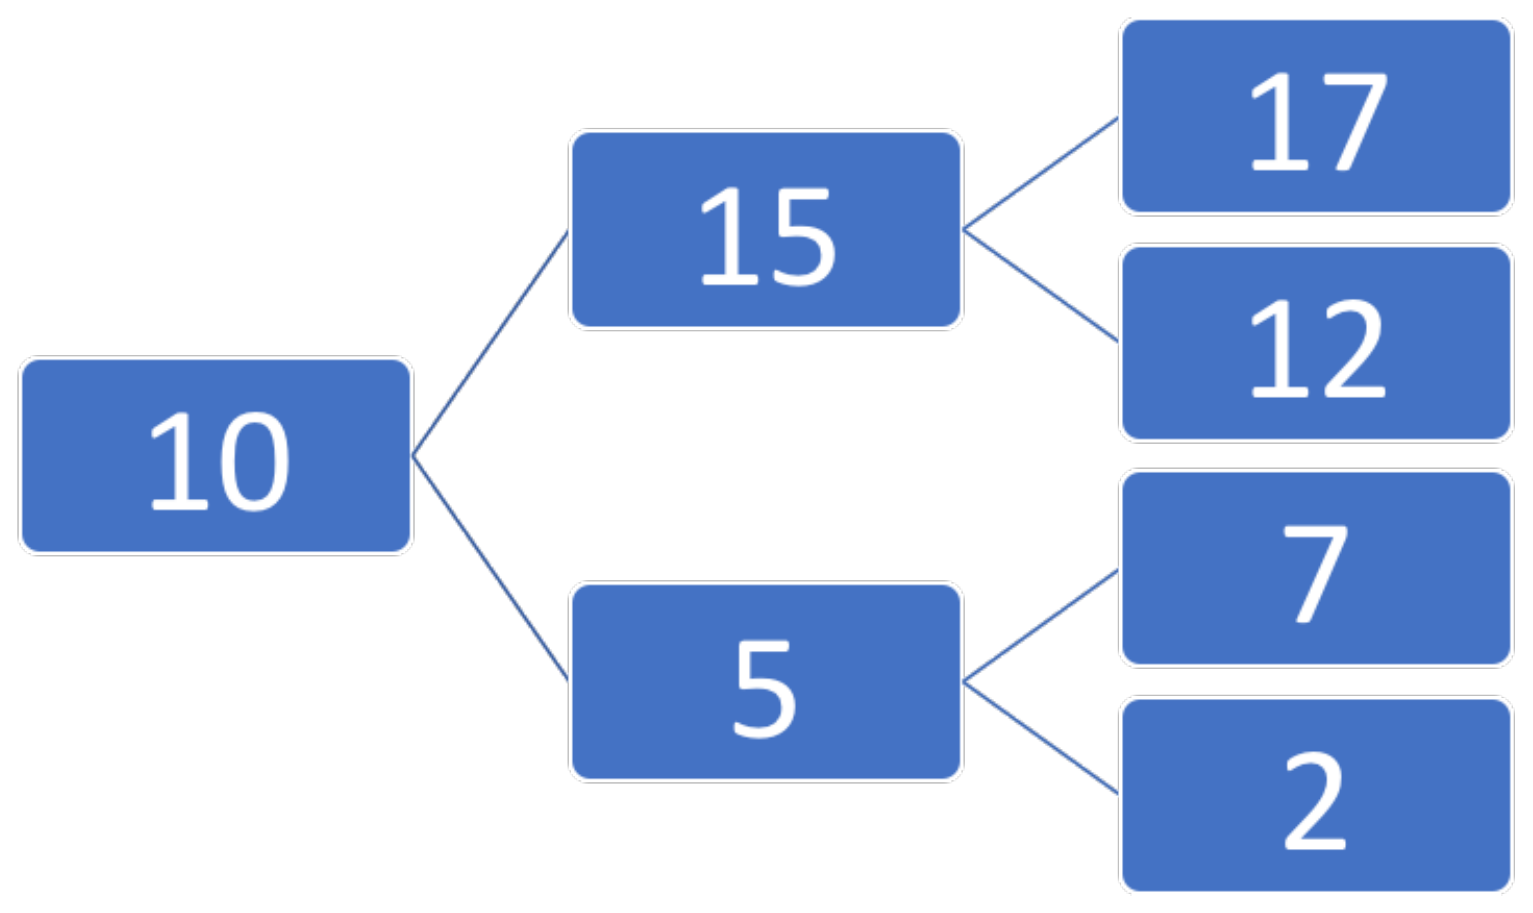
\includegraphics[scale=0.3]{map}

We iterator over it using this code (the values being displayed are
the key values for our map) 
\begin{lyxcode}
for(auto~i=map.begin();~i!=map.end();~i++)~

~~~cout~<\textcompwordmark{}<~{*}i~<\textcompwordmark{}<~endl;
\end{lyxcode}
We will get 
\begin{lyxcode}
2

5

7

10

12~

15~

17~
\end{lyxcode}
\item \textbf{Text Frequency} 

For the next part you are going to do some text frequency analysis.
You should create an object \texttt{textFrequencies}:

\texttt{my\_map<string,double>textFrequencies;}
\item \textbf{Reading File }

You should complete the \texttt{read\_file function}, which just reads
the whole file into one string. Next remove all of the punctuation
from the file using the \texttt{remove\_punctuation} function (this
is already done for you). 
\item \textbf{Counting} 

Complete the function \texttt{create\_freq\_map} which takes the string
that you generated previously and create the map from each word in
the text. First it would be useful to use a string stream for parsing
that big string of text. This will create a string stream for you
to use. 

\texttt{stringstream ss(text)} ;

Once you have that string stream you can use it just like a file stream
(or \texttt{cin})

\texttt{ss >\textcompwordmark{}> word; }

To do this you should use the brackets operator you implemented earlier.
The first step of this will pass over each word in the text and count
how many times you see that word, it would be helpful to use. 

\texttt{map{[}\textquotedbl{}word\textquotedbl{}{]}++} ;

Now after you have counted everything you need to divide each word
count by the total count of words in the text. First you need to find
every word in your map. To do this we will use iterators. If you implemented
your begin, end, and \texttt{++ operators} on your iterator properly
you should be able to use this for loop. 

\texttt{for(auto word: freq\_map);} 

That for loop will find every word in your map, and then you just
use this calculation to generate the frequency. 

\texttt{map{[}word{]} /=total\_cnt;}
\item \textbf{Output} 

Complete the \texttt{vectorize\_map} function, which translates your
map into a vector. This should use your \texttt{my\_map} iterators.
Next finish the \texttt{print\_top\_20\_freqs} function which should
print the 20 most frequent words. 
\item \textbf{Filter} 

You should notice that you see a lot of meaningless words (the, and,
of, for \dots ) in your top 20 words. To fix this, make a list of
words that you would want to filter out and remove them from your
frequency vector. 
\item \textbf{Analysis} 

Now print out your filtered output and create a table of words and
their frequencies. Finally make a plot of words on the x axis and
their frequencies on the y axis. 
\item \textbf{Hints }

All operations in your map should rely on operations from your binary
tree/vector, so for example don\textquoteright t try to rewrite the
insert function, because you already did it. Also if you look at the
start of your \texttt{my\_map}, you have a \texttt{BTree<key\_value<T,E>\textcompwordmark{}>},
which is the main data structure for your map, don\textquoteright t
try to change its type. \medskip{}
\item \textbf{Report}
\begin{enumerate}
\item Explain how your brackets operator works.
\begin{enumerate}
\item What is the running time expressed in terms of big-Oh asymptotic notation
of your brackets operator?
\item How could you improve the running time? Here don\textquoteright t
think about micro optimizations, think about changing data structures
or major algorithm changes. 
\end{enumerate}
\item Explain what the advantages and disadvantages of implementing map
with the following data structures 
\begin{enumerate}
\item A vector of key\_values b. 
\item A tree of key\_values. 
\begin{enumerate}
\item Regular binary
\item Red Black
\item AVL 
\item 2-4 
\end{enumerate}
\item A Hash Table of key\_values 
\end{enumerate}
\item Explain one real life use case for a map, you should say specifically
why it would benefit from using a map over a simpler data structure
like a vector. This doesn\textquoteright t have to be something that
exists currently, it\textquoteright s just an idea for how you could
use a map. Example (don\textquoteright t use this one) storing word
frequencies for a large document. 
\item Grading 

When we grade this, we will not be using your main file, we will be
using our own. Because of this do not change the file name that holds
the main function, also make sure you use a make file. When we grade
we will be making sure that you map does not crash/throw exceptions
under any circumstances. We will be taking some input from file and
storing them into your map, performing some operations using the brackets
operator, then printing the map out, your map should print in sorted
order. We will provide a \texttt{main} function that will test all
of the same operators, but with different inputs. 

\begin{tabular}{|c|c|}
\hline 
Points distribution & \tabularnewline
\hline 
Using PA4 Tree & 15\tabularnewline
\hline 
 Input/output operators  & 10\tabularnewline
\hline 
 Constructors & 5\tabularnewline
\hline 
Brackets adding & 5\tabularnewline
\hline 
Brackets searching & 5\tabularnewline
\hline 
Brackets search miss & 5\tabularnewline
\hline 
Brackets update & 5\tabularnewline
\hline 
Iterator \texttt{begin()/end()} & 10\tabularnewline
\hline 
Iterator \texttt{operator++} & 10\tabularnewline
\hline 
Report & 30\tabularnewline
\hline 
Total & 100\tabularnewline
\hline 
\end{tabular} 

\end{enumerate}
\end{itemize}

\section*{}
\begin{lyxcode}
\end{lyxcode}

\end{document}
